% !TeX root = ./pf.tex

%\includeonlyframes{current}

\section*{Elements of computer architecture}

\begin{frame}{The language of a computer}
  \begin{itemize}[<+->]
  \item A \textit{computer} is a device that executes programs
  \item A \textit{program} is a collection of instructions to perform a specific
    task
  \item For a computer to understand instructions, these need to be expressed in a
    language that the computer can understand
  \end{itemize}

\end{frame}

\begin{frame}{Many types of computers}

  \begin{columns}[b]

    \begin{column}{.5\textwidth}

      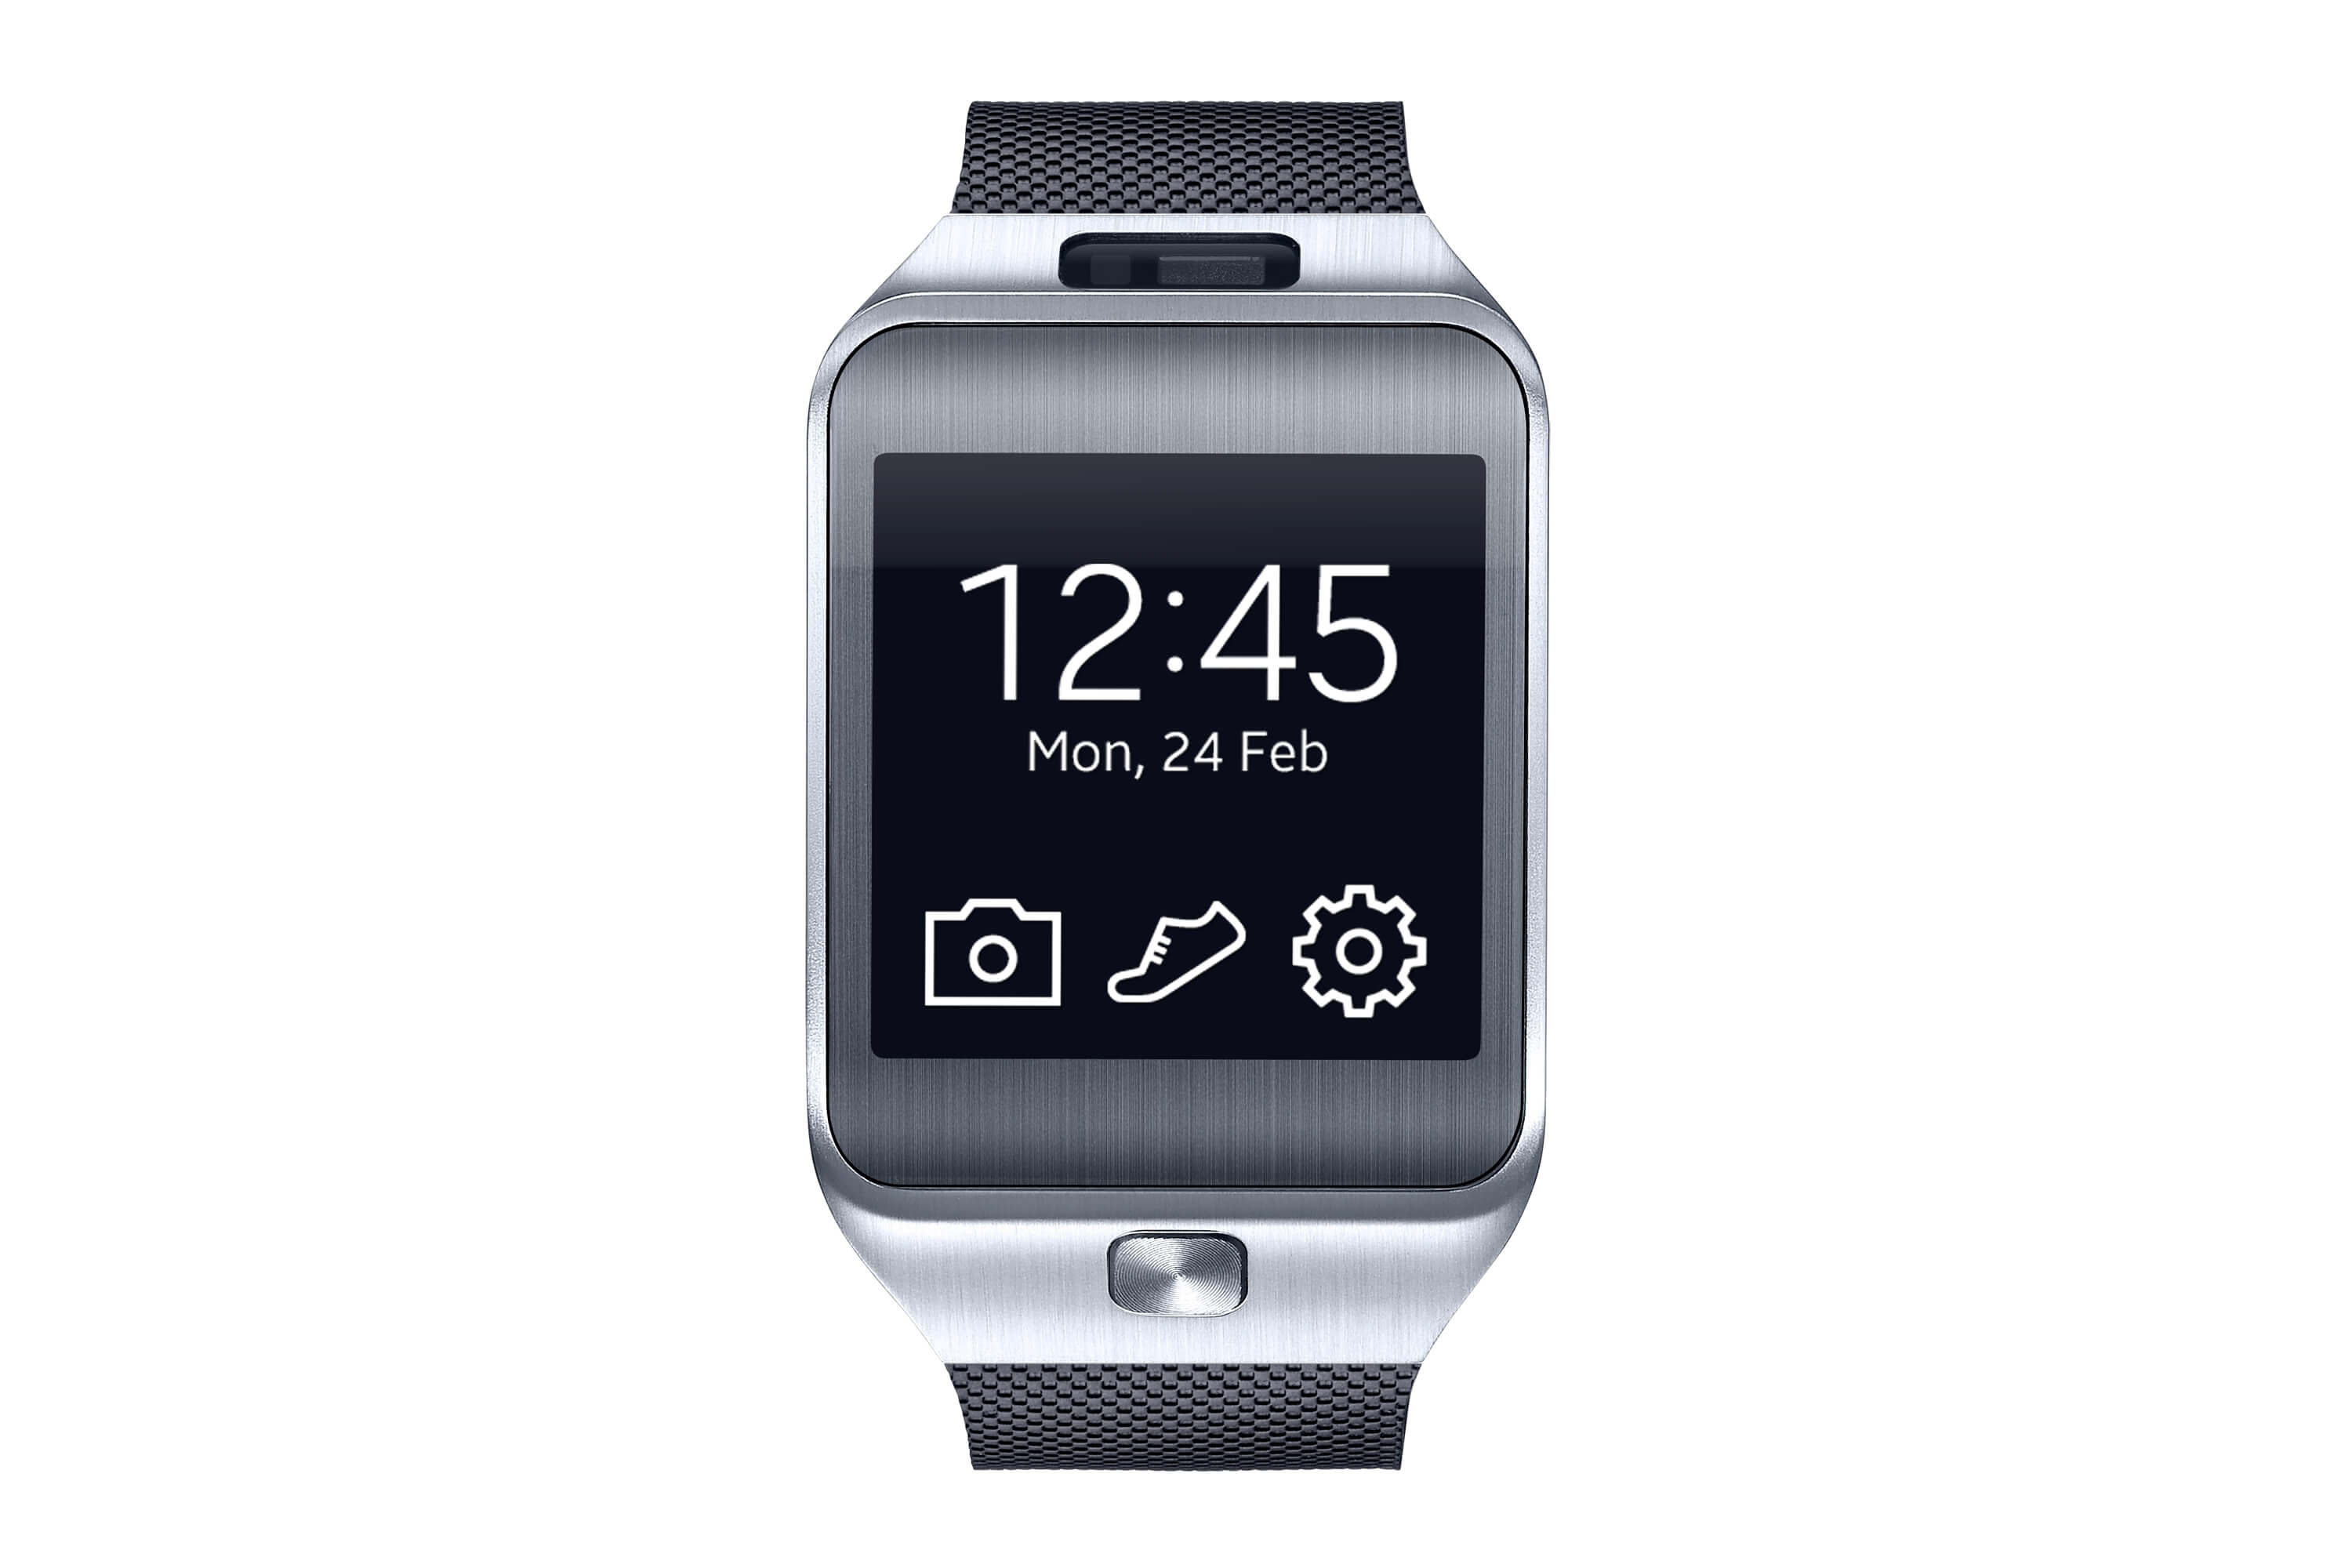
\includegraphics[width=\textwidth]{images/samsung-gear-compressed.jpeg}

      \begin{center}
        {\tiny(from \url{https://www.samsung.com/})}
      \end{center}
    \end{column}

    \begin{column}{.5\textwidth}
      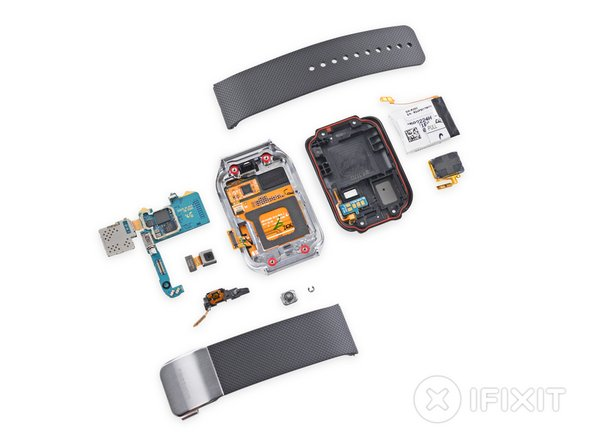
\includegraphics[width=\textwidth]{images/gear2-ifixit.jpg}

      \begin{center}
        {\tiny (from \url{https://www.ifixit.com/})}
      \end{center}
    \end{column}

  \end{columns}

\end{frame}

\begin{frame}{Many types of computers \insertcontinuationtext}
  \begin{columns}[b]
    \begin{column}{.5\textwidth}
      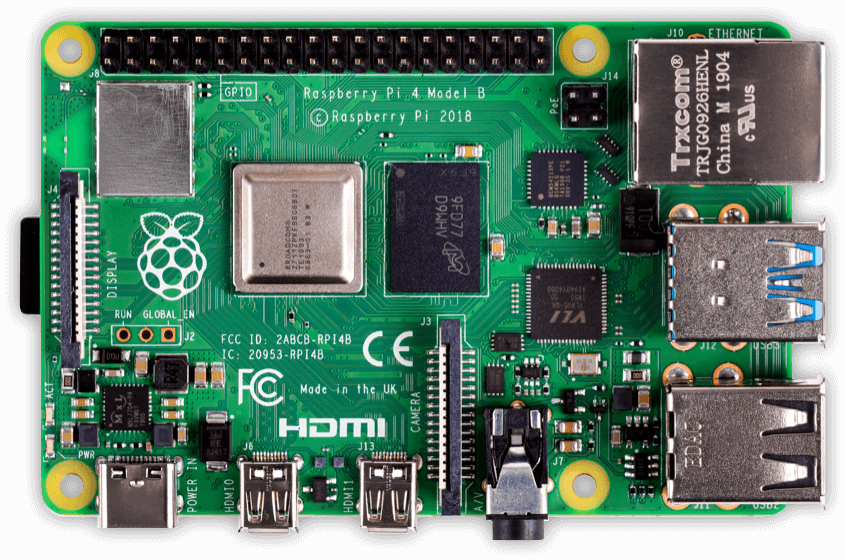
\includegraphics[width=\textwidth,angle=270,origin=c]{images/rpi-compressed.png}

      {\tiny (from \url{https://www.raspberrypi.org/})}
    \end{column}
    \begin{column}{.5\textwidth}
      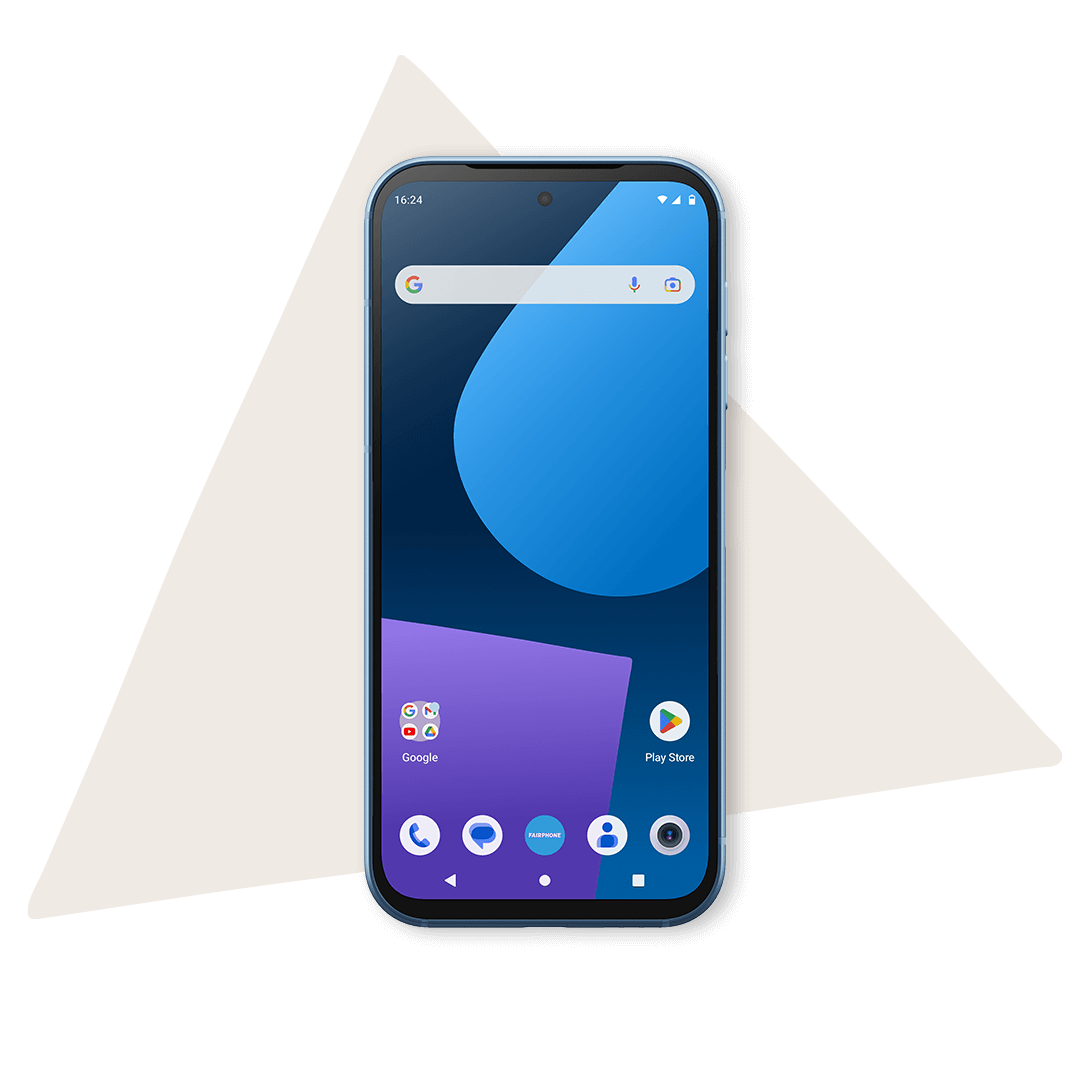
\includegraphics[trim={100 150 100 50},clip,width=\textwidth]{images/phone.png}
      {\tiny (from \url{https://www.fairphone.com/})}
    \end{column}
  \end{columns}
\end{frame}

\begin{frame}{Many types of computers \insertcontinuationtext}
  \begin{columns}
    \begin{column}{.5\textwidth}
  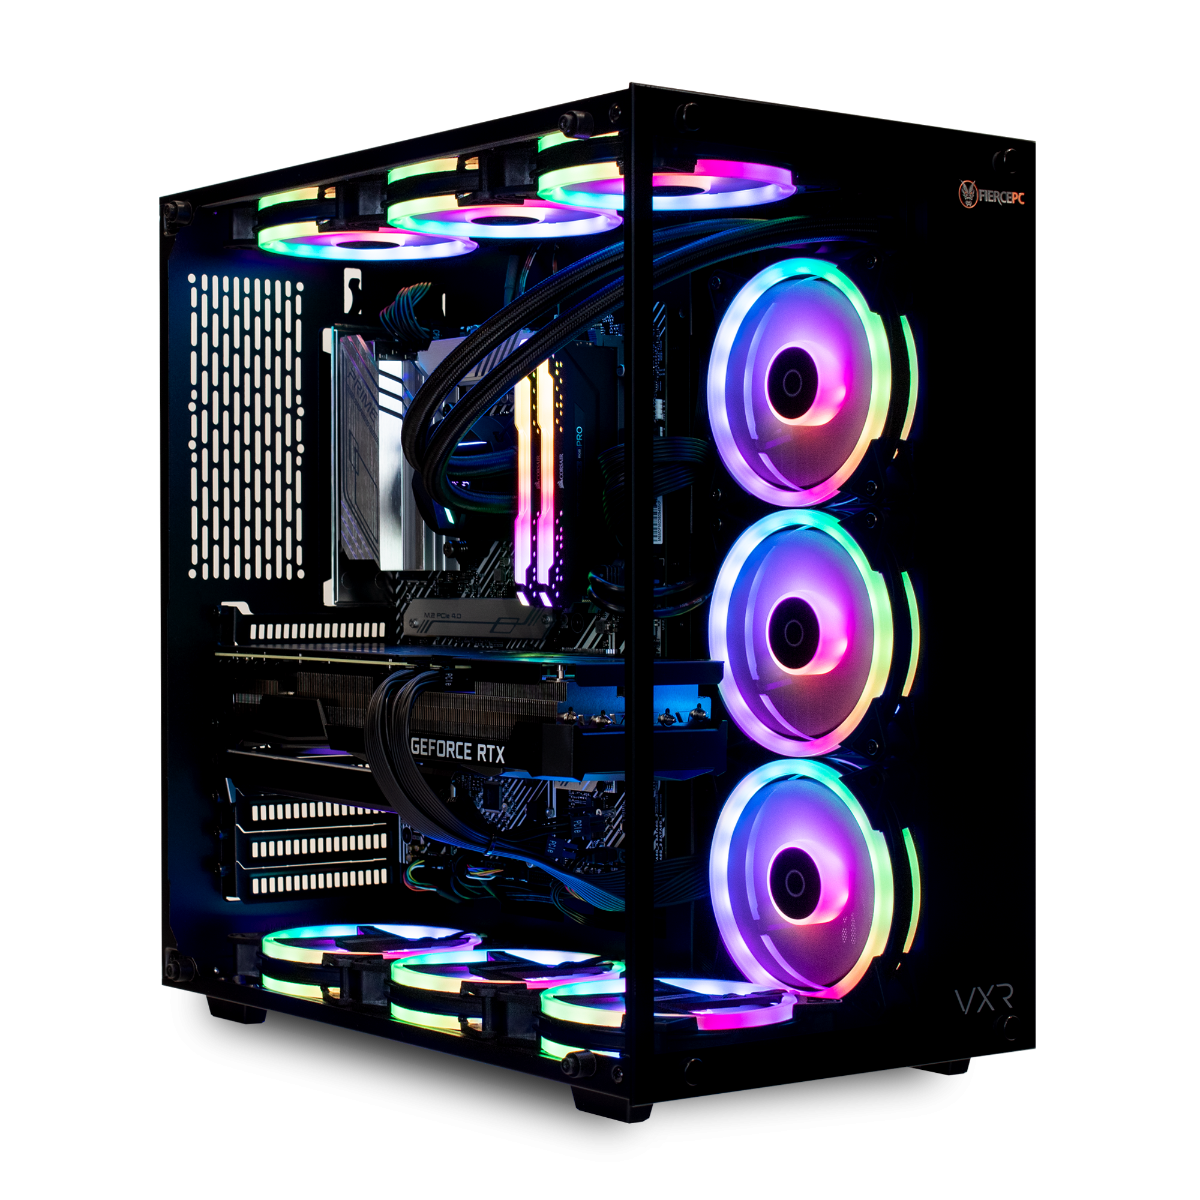
\includegraphics[width=\textwidth]{images/desktop.png}
    \end{column}
    \begin{column}{.5\textwidth}
  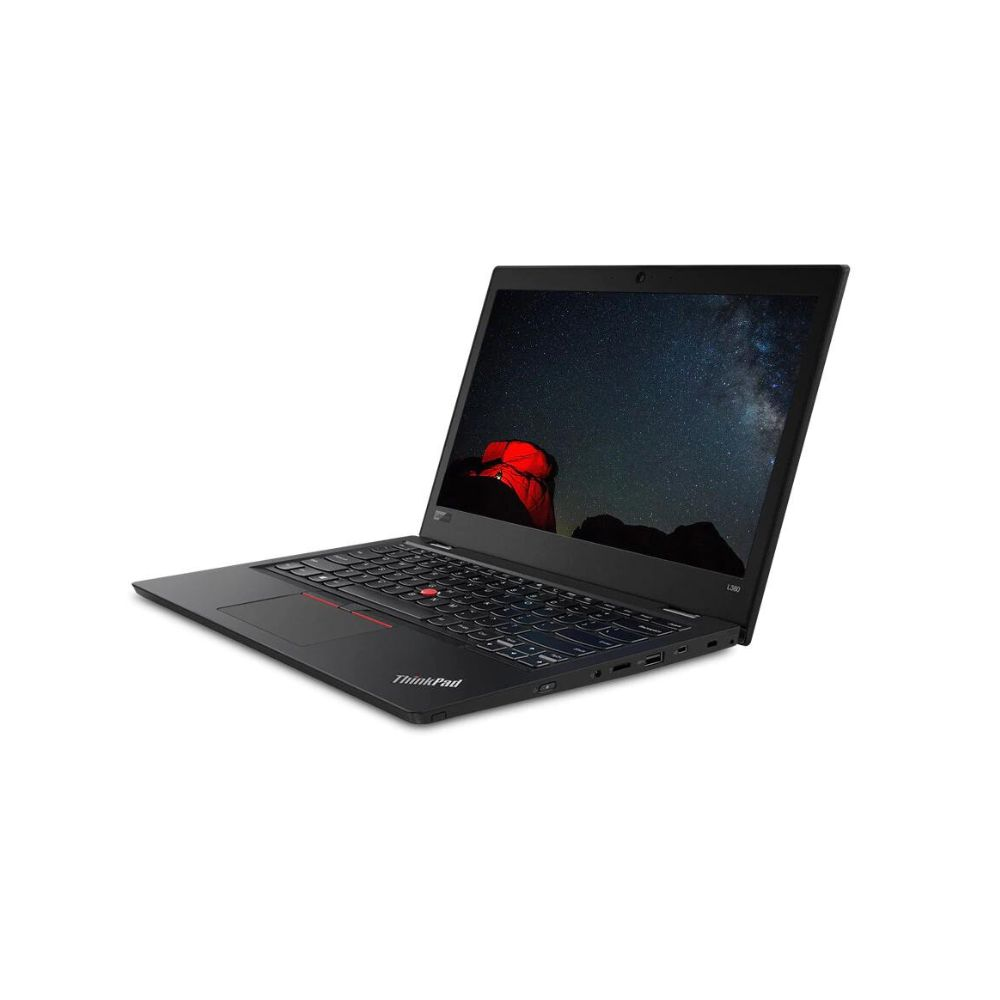
\includegraphics[width=\textwidth]{images/laptop.jpg}
    \end{column}
  \end{columns}
\end{frame}

\begin{frame}{Many types of computers \insertcontinuationtext}
  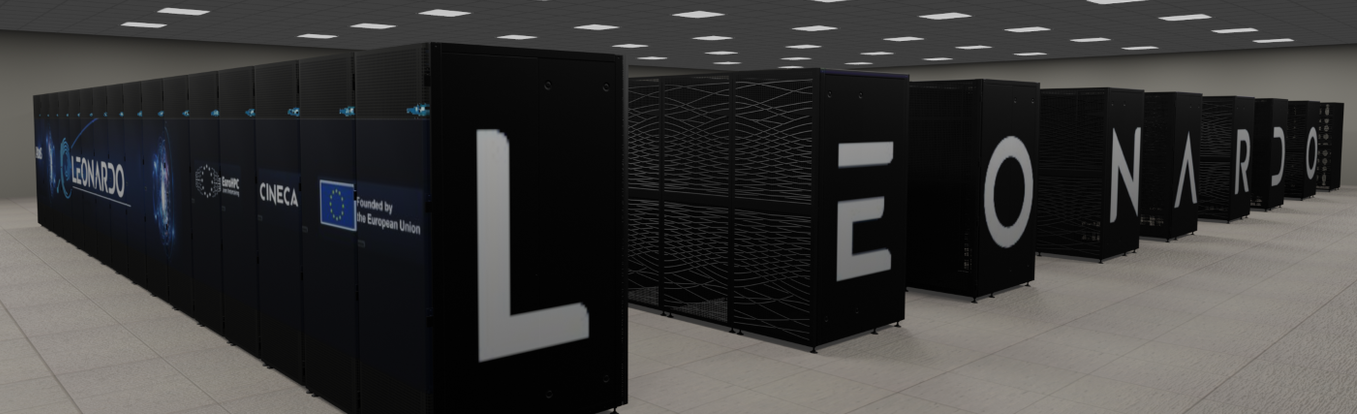
\includegraphics[width=\textwidth]{images/leonardo.png}

  {\tiny (from \url{https://wiki.u-gov.it/confluence/display/SCAIUS})}
\end{frame}

\begin{frame}[fragile]{Computers understand a binary language}

\begin{semiverbatim}
{\color{gray}\tikzref{markbit}0010\tikzref{markbyte}1001110110011000011111010111001011100111101100
11101000101001101011100111111100011101001000011010
00000110001101000011111010010001000101110000010010
00111011010111101101111110110011011111101100101101
10010010110011001101110011000011001011000001010010
11110100101111010001111001011000000000001111110100
1001110101100011010100\tikzref{ins}011100000001\tikzref{ins2}11000011\tikzref{ins3}01001101
00010001111001101000111100100110110110001101100100
01000110010111100011100010100101011011000110010001
10100011111101101000000000111101000001000100101101
11101100011010111001111110010101010110010010000100
00000010010011111010111011011101110011101100000111
00001001111011000000110000100110000101000100111011}\end{semiverbatim}

\uncover<2->{
  \uncover<2->{\tikz[overlay] \node[draw,rounded corners,thick,green,minimum
  width=3mm,minimum height=5mm,label={\color{green}bit}] (bit) at ([xshift=.5ex]markbit) {};}
  \uncover<3->{\tikz[overlay] \node[draw,rounded corners,thick,blue,minimum
  width=17mm,minimum height=7mm,label={45:{\color{blue}byte (8 bits)}}] (byte) at ([xshift=-.4ex]markbyte) {};}
  \uncover<4->{\tikz[overlay] \node[draw,rounded corners,thick,red,minimum width=49mm,minimum height=5mm] (instruction) at (ins) {};
  \tikz[overlay] \node[red] (description) at ([yshift=-32mm]instruction.south) {increment a number by 1 (for my laptop)};
  \tikz[overlay] \draw[<-,red,thick] (instruction) -- (description);}
}

\end{frame}

\begin{frame}[fragile]{Programming language}
  \begin{itemize}
  \item<1-> A (high-level) programming language is an artificial language to write
    programs that is closer to humans
    \begin{codeblock}
int increment(int n)
\{
  return n + 1;
\}\end{codeblock}        
  \item<1-> More or less equivalent to the mathematical function
  \[
    \verb|increment|(n) = n + 1 \quad \forall n \in \mathbb{Z}
  \]

  \item<2-> Some form of translation needs to be applied to the program written in a
    high-level language to transform it into a program expressed in a binary
    language
    \begin{itemize}
    \item A program expressed in a binary language is usually called \textit{executable}
    \end{itemize}
  \end{itemize}

\end{frame}
\begin{frame}[fragile]{Programming language \insertcontinuationtext}
  \begin{itemize}
  \item<1-> To complicate things, the binary language is computer-specific (the
    correct term is \textit{architecture}-specific)
    \begin{itemize}[<.->]
    \item An Instruction Set Architecture (ISA) defines, among other things, the
      binary instructions understood by a computer implementing that
      architecture
    \item Many ISAs have been defined over the years, many still in use
    \item i386, \textbf{x86_64}, SPARC, MIPS, \textbf{ARM}, VAX, Alpha, RiscV,
      PowerPC, \ldots
    \end{itemize}
  \item<2-> The translation from high-level language to binary language is done
    by other programs
    \begin{itemize}[<.->]
    \item \alert{compilers} and interpreters
    \end{itemize}
  \end{itemize}

\end{frame}

\begin{frame}{The Von Neumann architecture}

  Despite their differences, all architectures are inspired at the architecture
  first described by John Von Neumann in 1945.

  \begin{center}

    \vskip -.4cm

    \begin{tikzpicture}[every text node part/.style={align=center}]
      \uncover<3->{
        \node[rectangle,draw,thick,minimum height=4cm,minimum width=2.1cm,fill=yellow,"Memory"] (memory) {
          data \\ + \\ instructions
        };
        \node[above=20pt of memory,inner sep=0pt,outer sep=0pt] (ram) {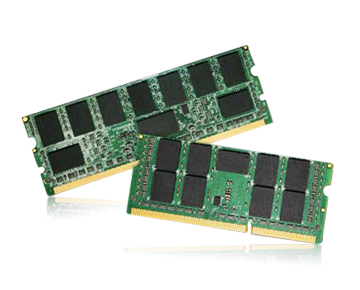
\includegraphics[height=1cm]{images/ram.jpg}};
      }
      \uncover<2->{
        \node[rectangle,black,draw,thick,minimum height=4cm,minimum width=2.5cm,fill=red!80!black,right=of memory,"CPU"] (cpu) {};
        \node[rectangle,black,draw,thick,text width=2cm,minimum
        height=1cm,fill=white,below=10pt of cpu.north,inner sep=0pt,outer sep=0pt] (alu) {\scriptsize
          Arithmetic-Logic Unit};
        \node[rectangle,black,draw,thick,minimum width=2cm,fill=white,above=of cpu.south] (control) {\scriptsize Control};
        \path (alu) -- (control) node[midway,rectangle,black,draw,thick,minimum width=2cm,fill=white] (registers) {\scriptsize Registers};
        \node[above=20pt of cpu,inner sep=0pt,outer sep=0pt] (intel) {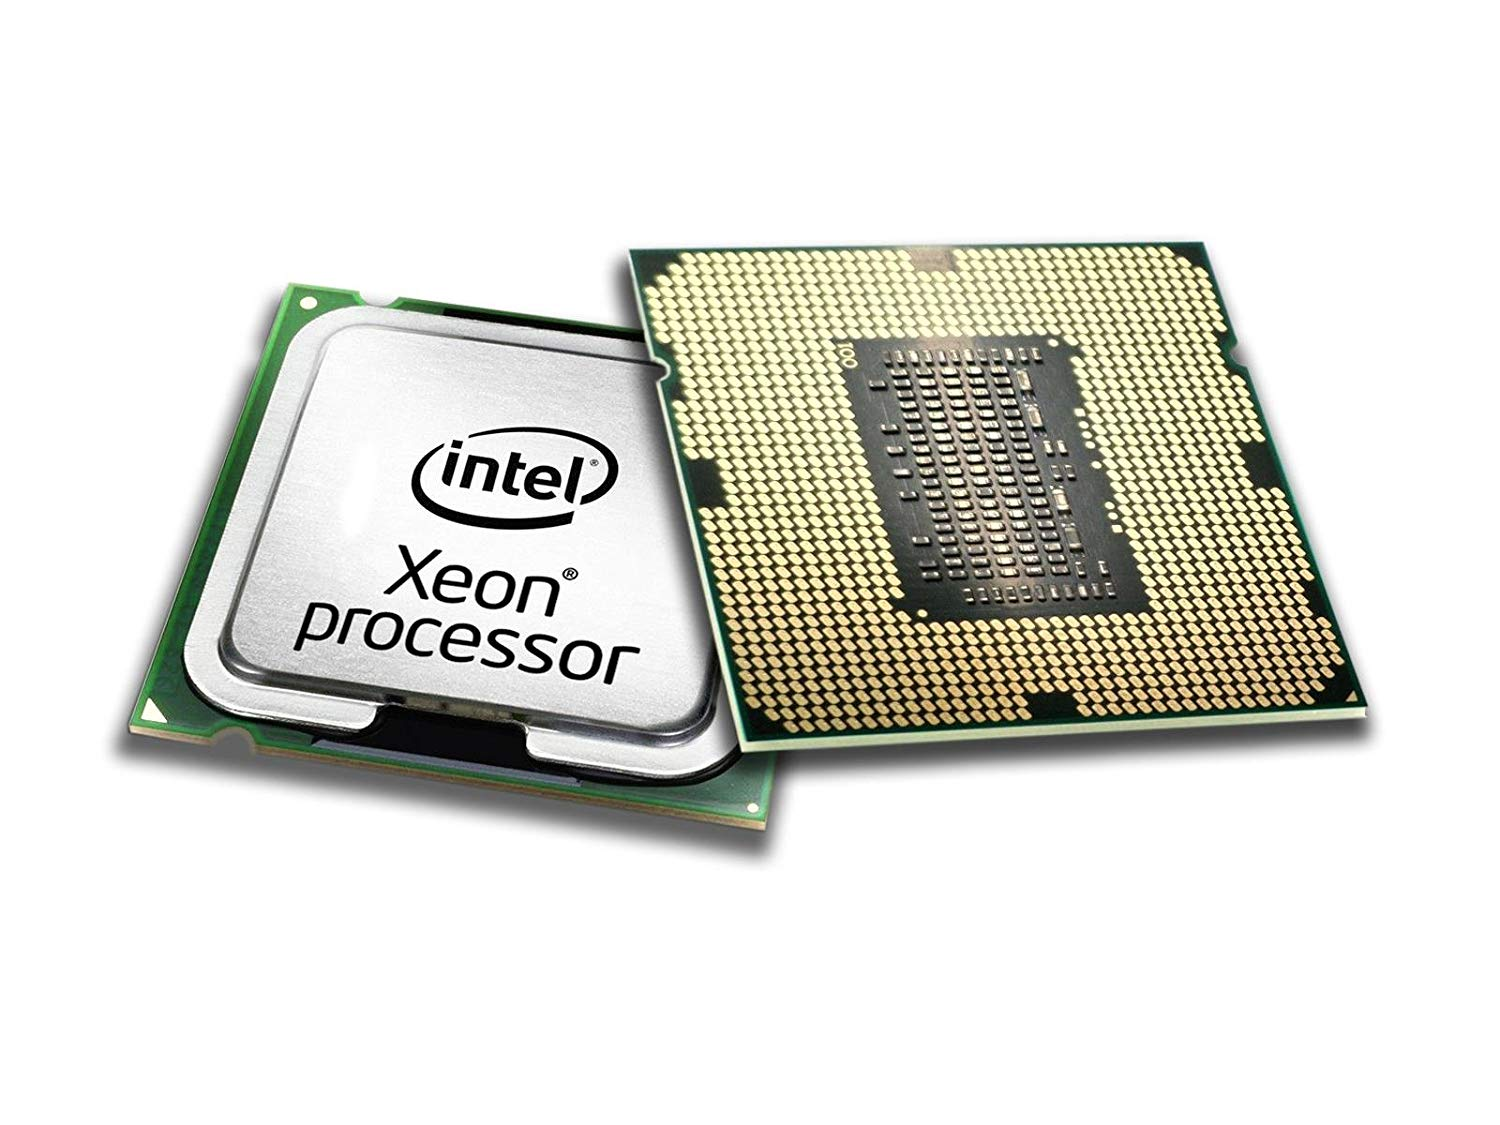
\includegraphics[height=1cm]{images/cpu.jpg}};
      }
      \uncover<3->{\draw[<->,thick] (memory) -- (cpu);}
      \uncover<4->{
        \node[tape,draw,thick,minimum height=1.5cm,minimum width=2cm,fill=green,right=of cpu.north east,yshift=-1cm] (input) {Input};
        \node[tape,draw,thick,minimum height=1.5cm,minimum width=2cm,fill=green,right=of cpu.south east,yshift=1cm] (output) {Output};
        \draw[<-,thick] (cpu) -- (input);
        \draw[->,thick] (cpu) -- (output);
        \node[above=20pt of input,outer sep=0pt,inner sep=0pt] (keyboard) {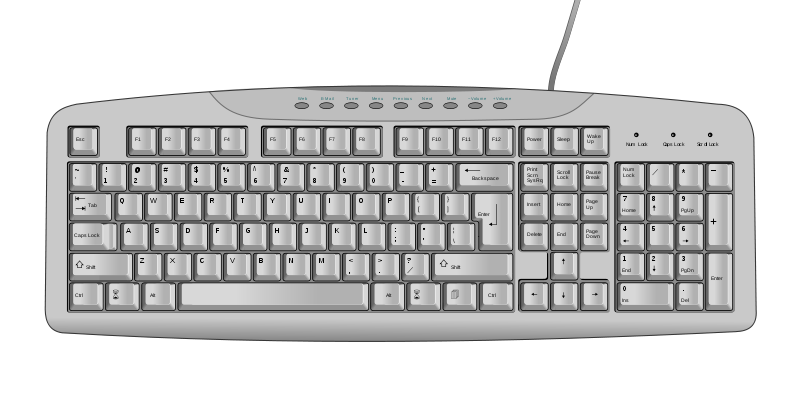
\includegraphics[height=1cm]{images/keyboard.png}};
        \node[right=0pt of keyboard] (mouse) {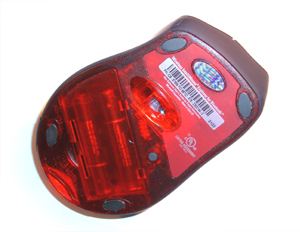
\includegraphics[height=1cm]{images/mouse.jpg}};
        \node[below right=0pt and 0pt of mouse,xshift=-.5cm] (monitor) {
\includegraphics[height=1cm]{images/monitor.png}};
        \node[below=0pt of monitor] (harddisk) {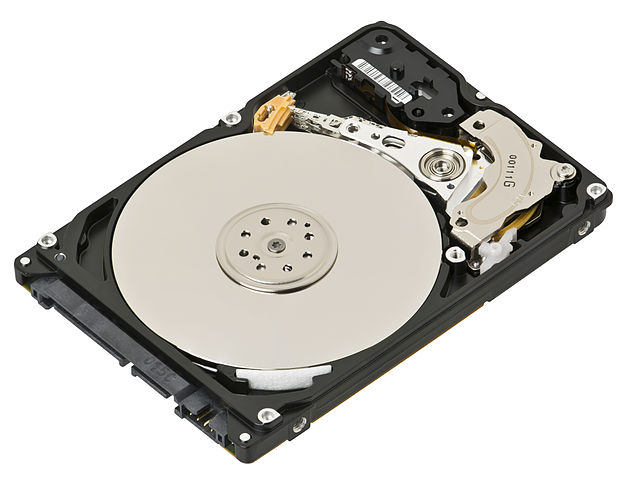
\includegraphics[height=1cm]{images/harddisk.jpg}};
        \node[below=0pt of harddisk] (usb-stick) {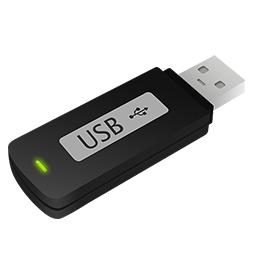
\includegraphics[height=1cm]{images/usb-stick.png}};
        \node[below=0pt of usb-stick] (router) {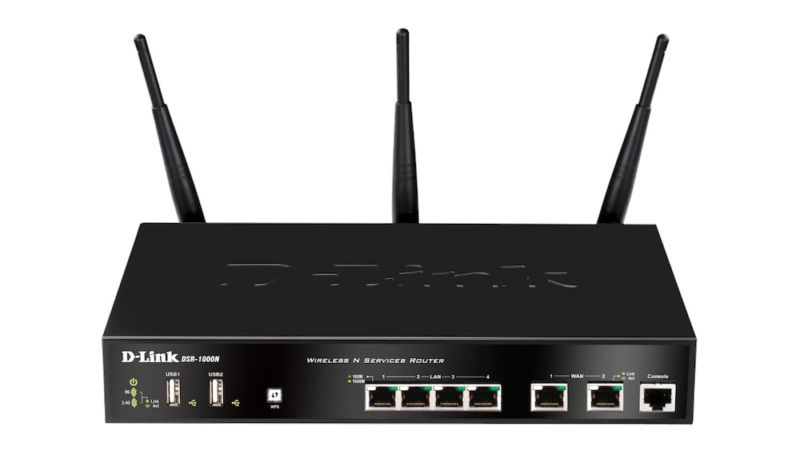
\includegraphics[height=1cm]{images/router.jpg}};
        \node[below left=-20pt and 10pt of router] (gpu) {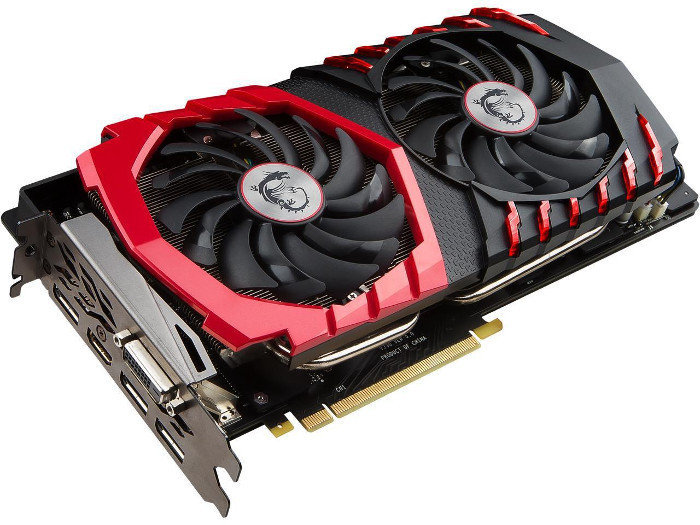
\includegraphics[height=1cm]{images/gpu.jpg}};
        \node[left=0pt of gpu] (sensor) {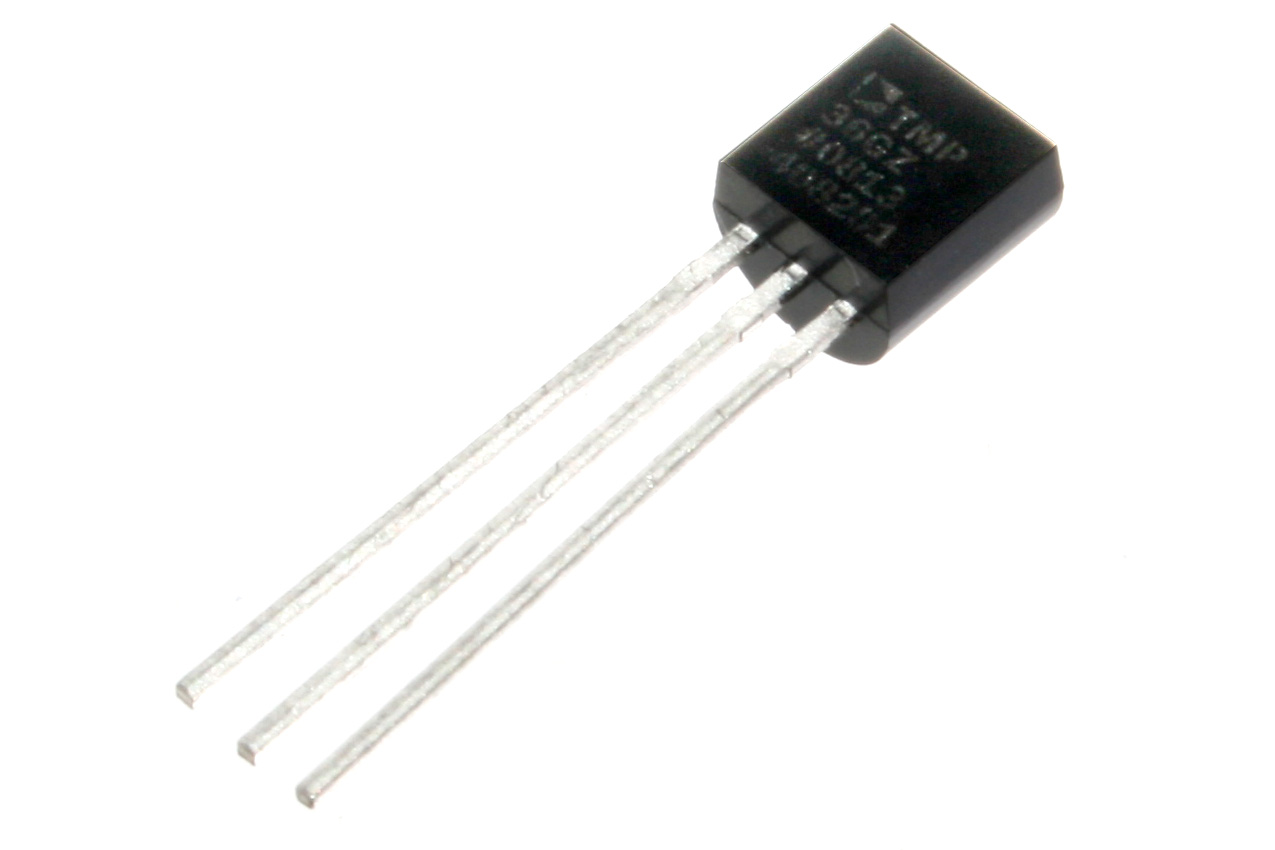
\includegraphics[height=1cm]{images/sensor.jpg}};
      }
    \end{tikzpicture}
  \end{center}

\end{frame}

\begin{frame}{The Von Neumann architecture \insertcontinuationtext}

  \begin{itemize}[<+->]
  \item Imagine memory as a looooong tape divided into locations whose content
    you can read and write
    \begin{itemize}[<.->]
    \item Each location has the same size (let's assume one byte, i.e. 8 bits)
    \item A piece of data can occupy multiple locations
    \end{itemize}
  \item Each memory location is identified by an index
    \begin{itemize}[<.->]
    \item e.g. location at position 8'363'944
    \end{itemize}
  \item During execution, executables (i.e. binary programs) and the data they
    manage stay both in memory, typically in different regions
  \item The CPU fetches binary instructions from memory into its registers and
    executes them
  \item Typical instructions:
    \begin{itemize}[<.->]
    \item read data (e.g. a number) from a memory location into a register
    \item write data (e.g. a number) from a register to a memory location
    \item manipulate data (e.g. increment a number or add two numbers) in
      registers
    \end{itemize}
  \end{itemize}
\end{frame}

\begin{frame}[fragile]{Also data are binary}

  \begin{semiverbatim}
{\color{gray}...01001110110011000011111010111001011100111101100
11101000101001101011100111111100011101001000011010
00000110001101000011111010010001000101110000010010
00111011010111101101111110110011011111101100101101
10010010110011001101110011000011001011000001010010
11110100101111010001111001011000000000001111110100
1001110110001101101001\tikzref{ins}0110000101101111000000001101
00010001111001101000111100100110110110001101100100
01000110010111100011100010100101011011000110010001
10100011111101101000000000111101000001000100101101
00001001111011000000110000100110000101000100111...}\end{semiverbatim}

\uncover<2->{
  \tikz[overlay] \node[draw,thick,rounded corners,red,minimum width=65mm,minimum
  height=5mm] (data) at (ins) {};
}

\begin{itemize}
\item<3-> read as \alert<3>{integer number}, the value is $1667850607$
\item<4-> read as \alert<4>{floating-point number}, the value is $4.30511 \times 10^{21}$
\item<5-> read as \alert<5>{character string}, the value is ``ciao''
\end{itemize}
\end{frame}
